%%%%%%%%%%%%%%%%%%%%%%%%%%%%%%%%%%%%%%%%%
% Journal Article
% LaTeX Template
% Version 1.3 (9/9/13)
%
% This template has been downloaded from:
% http://www.LaTeXTemplates.com
%
% Original author:
% Frits Wenneker (http://www.howtotex.com)
%
% License:
% CC BY-NC-SA 3.0 (http://creativecommons.org/licenses/by-nc-sa/3.0/)
%
%%%%%%%%%%%%%%%%%%%%%%%%%%%%%%%%%%%%%%%%%

%----------------------------------------------------------------------------------------
%    PACKAGES AND OTHER DOCUMENT CONFIGURATIONS
%----------------------------------------------------------------------------------------

\documentclass[twoside]{article}

\usepackage{lipsum}
\usepackage{graphicx}

\usepackage{listings}
\usepackage{color}

\lstset{
    language=Java,                % choose the language of the code
    basicstyle=\footnotesize,       % the size of the fonts that are used for the code
    numbers=left,                   % where to put the line-numbers
    numberstyle=\footnotesize,      % the size of the fonts that are used for the line-numbers
    stepnumber=1,                   % the step between two line-numbers. If it is 1 each line will be numbered
    numbersep=5pt,                  % how far the line-numbers are from the code
    backgroundcolor=\color{white},  % choose the background color. You must add \usepackage{color}
    showspaces=false,               % show spaces adding particular underscores
    showstringspaces=false,         % underline spaces within strings
    showtabs=false,                 % show tabs within strings adding particular underscores
    frame=single,           % adds a frame around the code
    tabsize=2,          % sets default tabsize to 2 spaces
    captionpos=b,           % sets the caption-position to bottom
    breaklines=true,        % sets automatic line breaking
    breakatwhitespace=false,    % sets if automatic breaks should only happen at whitespace
    escapeinside={\%*}{*)}          % if you want to add a comment within your code
}

\usepackage[sc]{mathpazo} % Use the Palatino font
\usepackage[T1]{fontenc} % Use 8-bit encoding that has 256 glyphs
\linespread{1.05} % Line spacing - Palatino needs more space between lines
\usepackage{microtype} % Slightly tweak font spacing for aesthetics

\usepackage[hmarginratio=1:1,top=32mm,columnsep=20pt]{geometry} % Document margins
\usepackage{multicol} % Used for the two-column layout of the document
\usepackage[hang, small,labelfont=bf,up,textfont=it,up]{caption} % Custom captions under/above floats in tables or figures
\usepackage{booktabs} % Horizontal rules in tables
\usepackage{float} % Required for tables and figures in the multi-column environment - they need to be placed in specific locations with the [H] (e.g. \begin{table}[H])
\usepackage{hyperref} % For hyperlinks in the PDF

\usepackage{lettrine} % The lettrine is the first enlarged letter at the beginning of the text
\usepackage{paralist} % Used for the compactitem environment which makes bullet points with less space between them

\usepackage{abstract} % Allows abstract customization
\renewcommand{\abstractnamefont}{\normalfont\bfseries} % Set the "Abstract" text to bold
\renewcommand{\abstracttextfont}{\normalfont\small\itshape} % Set the abstract itself to small italic text

\usepackage{titlesec} % Allows customization of titles
\renewcommand\thesection{\Roman{section}} % Roman numerals for the sections
\renewcommand\thesubsection{\Roman{subsection}} % Roman numerals for subsections
\titleformat{\section}[block]{\large\scshape}{\thesection.}{1em}{} % Change the look of the section titles
\titleformat{\subsection}[block]{\large}{\thesubsection.}{1em}{} % Change the look of the section titles

\usepackage{fancyhdr} % Headers and footers
\pagestyle{fancy} % All pages have headers and footers
\fancyhead{} % Blank out the default header
\fancyfoot{} % Blank out the default footer
\fancyhead[C]{Design Milestone $\bullet$ 6.005 Project 2 $\bullet$ 2013 Dec 3} % Custom header text
\fancyfoot[RO,LE]{\thepage} % Custom footer text

%----------------------------------------------------------------------------------------
%    TITLE SECTION
%----------------------------------------------------------------------------------------

\title{\vspace{-15mm}\fontsize{24pt}{10pt}\selectfont\textbf{Design Milestone}} % Article title

\author{
\large
\textsc{Andre Aboulian, Cathleen Gendron, \& Jon Beaulieu}\\[2mm] % member name
\normalsize 6.005 Software Construction - Fall 2013 - Project 2: "Collaborative Whiteboard"
\vspace{-5mm}
}
\date{}

%----------------------------------------------------------------------------------------

\begin{document}

\maketitle % Insert title

\thispagestyle{fancy} % All pages have headers and footers

\hspace{10mm}

\section{User Functionality Abstract}

\subsection{Components}

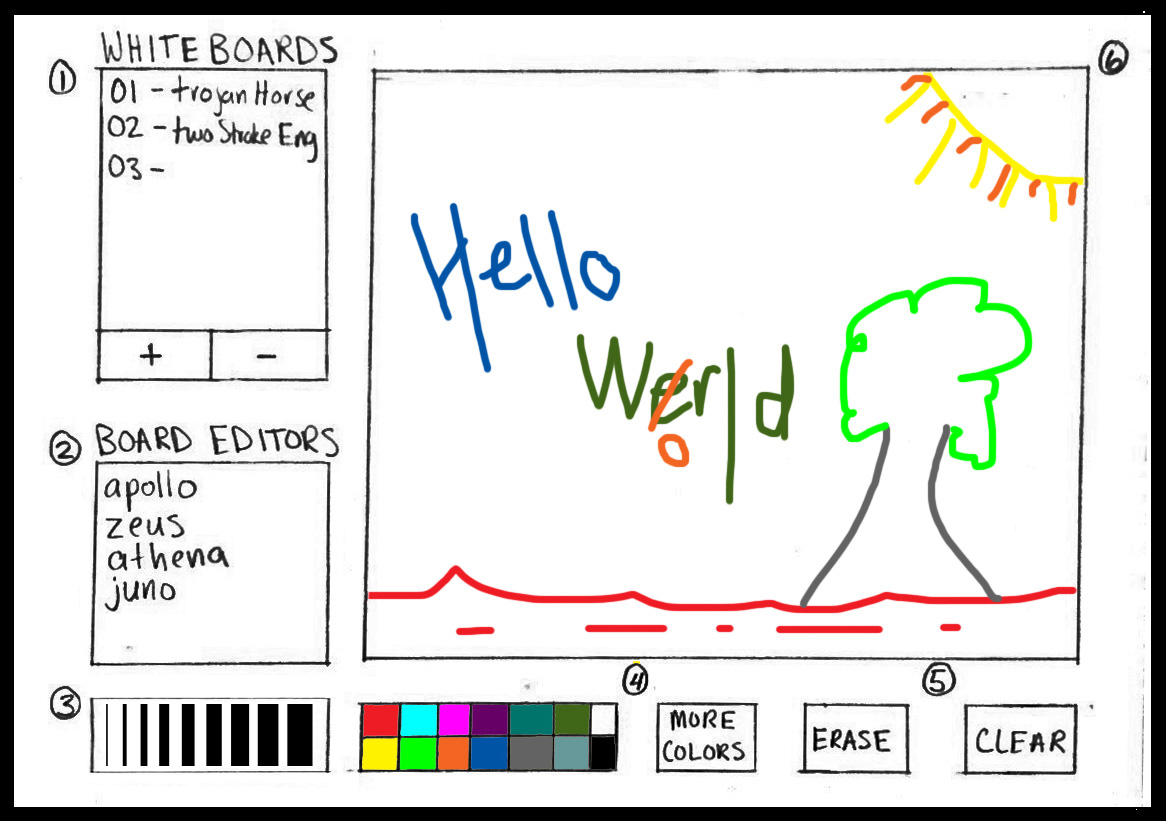
\includegraphics[keepaspectratio=1,width=6in]{img/gui-sketch.jpg}

\subsubsection{Selector}

The board selector in the left pane includes a list of all current whiteboards and appears the same for all users. Each line represents an individual board, which are numbered sequentially and named by the user. Upon clicking the "+" button, the user will be prompted to name the new board. When the board has been created on the server, it will be appended to the list for each user. Selecting a board in the list will download the board from the server, overwrite the local copy if one exists, and display the board in the canvas window. 

\subsubsection{Board Editors}

Displays a list of users, including the viewer, who are currently modifying the selected board. This list will be updated as users enter and exit the board.

\subsubsection{Thickness Selector}

This tool allows the user to select a brush/eraser thickness for drawing on the whiteboard.

\subsubsection{Color Selector}

The main color palette displays a grid of colors from which the user can choose to paint with. The color currently in use will be highlighted. Clicking the "more colors" button will open Swing's built-in color chooser, which will offer a larger selection of colors.

\subsubsection{Erasing Tools}

The erase button will allow the user to toggle between erasing and painting. "Erasing" will be defined as drawing with a white selection. Erasing will happen in the same order as drawing, so whichever request reaches the server first will erase all that has been drawn under it. Toggling back to painting will restore the user's previous color choice.

\subsubsection{Whiteboard Window}

Displays the currently selected whiteboard, including all of its drawn strokes and erasures. The whiteboard be real-time interactive to allow users to collaborate simultaneously. Edits will be made in the order that modifications reach the server. In other words, a stroke logged on the server at a specific instant will be drawn over any strokes drawn before that instant.

\subsection{Behavior}

\paragraph{Erasing}

Because the default canvas color is white, erasing will function the same as drawing with the color white selected.  The thickness functionality that is present during normal drawing will continue to work with erasing. The Erase button on the client GUI will function as a toggle. Clicking the button once will switch to erasing mode, which essentially is simply switching the client's selected color to white. At this time, the user's previously selected color will be stored for future use. Clicking the button a second time will return the user's selected color to what is was before the user entered erasing mode.

\paragraph{Editing a Deleted Board}

Clients should not be allowed to edit a board that has been deleted by another user. To prevent this, users who are working on a board when it is marked for deletion by another user will be presented with a message box, stating that their board has been deleted.  The deleted board then becomes unselected by any client GUIs who had the board selected at the time of deletion, forcing users to select a different whiteboard to work on. Simultaneously, the board will be removed from the master list of whiteboards available, so that no users in the future may accidentally select the deleted board.

\section{Server-Client Communication}

\subsection{Protocol}

\subsubsection{Grammar}
The following grammar will facilitate the text-based communication between the clients and the server. The server will send \texttt{StoC\_MSG} messages to the client, which will be able to send \texttt{CtoS\_MSG} messages back to the server.

\vspace{5mm}

\setlength{\parindent}{0in}

\texttt{StoC\_MSG :== (STROKE | BRD\_INFO | BRD\_DEL | USER\_INIT | BRD\_USERS) N}\\

\texttt{CtoS\_MSG :== (STROKE | SEL | BRD\_REQ | BRD\_DEL | BRD\_ALL | USER\_REQ) N}\\


\texttt{STROKE :== "stroke" S BOARD\_ID S THICK S COORDS S COLOR}\\
\texttt{COORDS :== X1 S Y1 S X2 S Y2}\\
\texttt{X1, Y1, X2, Y2 :== INT}\\
\texttt{COLOR :== [0-255] S [0-255] S [0-255]}\\
\texttt{THICK :== [1-10]}\\

\texttt{SEL :== "select" S BOARD\_ID}\\

\texttt{BRD\_REQ :== "board\_req" S NAME}\\
\texttt{BRD\_ALL :== "board\_all"}\\
\texttt{BRD\_INFO :== "board" S BOARD\_ID S NAME}\\
\texttt{BRD\_DEL :== "del" S BOARD\_ID}\\
\texttt{BRD\_USERS :== "board\_users" S BOARD\_ID (S USER\_NAME)+}\\

\texttt{USER\_REQ :== "user\_req" S USER\_NAME}\\
\texttt{USER\_INIT :== "you\_are" S USER\_NAME}\\

\texttt{NAME :== [$\char`\^$N]}\\
\texttt{USER\_NAME :== [A-Za-z]([A-Za-z0-9]?)+}\\
\texttt{BOARD\_ID :== INT}\\

\texttt{INT :== [0-9]+}\\
\texttt{N :== "$\backslash$r?$\backslash$n"}\\
\texttt{S :== " "}\\

\setlength{\parindent}{15pt} %default

\subsubsection{Definitions and Usage}
Below is the definition for each of the messages that can be sent across the network. Note that particular messages warrant a response after processing, and those returned messages are included in the definition.

\paragraph{\texttt{STROKE}} A \texttt{STROKE} message is sent from a client to the server upon drawing a line.
\begin{enumerate}
\item A \texttt{WhiteLine} object is created for the line from (\texttt{X1},\texttt{Y1}) to (\texttt{X2},\texttt{Y2}) with thickness \texttt{THICK} and color \texttt{COLOR}. It is then added to the \texttt{MasterBoard} corresponding to the provided \texttt{BOARD\_ID}.
\item The \texttt{STROKE} message is forwarded to all clients who are currently editing the same board, so that the line can be incorporated onto their whiteboards.
\end{enumerate}

\paragraph{\texttt{SEL}} Upon selecting a different board, the client sends a \texttt{SEL} request to the server.
\begin{enumerate}
\item The server clears all stroke messages queued to update the client's whiteboard.
\item The server disassociates the client with the current whiteboard if one is assigned and associates the client with the requested board.
\item A \texttt{BRD\_USERS} message is sent to all users of the requested board, with the addition of the new editor, to inform them of the change. Another \texttt{BRD\_USERS} message is sent to all users of the previous board, with the omission of the removed editor, to inform them of the change.
\item A sequence of \texttt{STROKE} messages are sent to the client to recreate the current state of the selected whiteboard.
\end{enumerate}

\paragraph{\texttt{BRD\_REQ}} When the client wants to create a new board, it send a \texttt{BRD\_REQ} message with a properly formatted \texttt{NAME}.
\begin{enumerate}
\item The server initializes a new \texttt{MasterBoard} object with relevant properties and adds it to its list of boards.
\item A \texttt{BRD\_INFO} message for the new board is sent to all connected clients to inform them of the newly available whiteboard. The clients add this board to their list of available boards.
\end{enumerate}

\paragraph{\texttt{BRD\_ALL}} This is often called by the client upon initialization. It prompts a series of \texttt{BRD\_INFO} replies for all existing boards.

\paragraph{\texttt{BRD\_DEL}} When the client wants to remove a board, it send a \texttt{BRD\_DEL} message to the server.
\begin{enumerate}
\item If the provided \texttt{BOARD\_ID} exists, the server removes the designated board from its central list of boards.
\item The \texttt{BRD\_DEL} message is forwarded to all clients to signify that the board is no longer available. The clients remove this board from their list of available boards.
\end{enumerate}

\paragraph{\texttt{USER\_REQ}} Upon entering a username in the client application, a \texttt{USER\_REQ} message with a properly formatted \texttt{USER\_NAME} will be sent to the server to request the desired username.
\begin{enumerate}
\item The requested username is checked against existing username. If the name already exists, a name is generated using the new board's ID number.
\item A \texttt{User} object with relevant properties is created to represent the new client.
\item A \texttt{USER\_INIT} message is sent to the client to inform it of its acquired username.
\end{enumerate}

Note that \texttt{BRD\_USERS}, \texttt{BRD\_INFO}, and \texttt{USER\_INIT} are used solely as replies and are included in the descriptions above.


\subsection{Data Transport}
For a detailed explanation of the communication method between the clients and the server, please see the "Threads and Queues" section.

\end{document}
